%%%%%%%%%%TO FORMAT A PREPRINT FOR A PCI%%%%%%%%%%%%%%%%
%%%%%%%%%%%%%%%%%%%%%%%%%%%%%%%%%%%%%%%%%%%%%%

\documentclass[a4paper]{article}
%%%%%%%%%   CHOOSE A PCI   %%%%%%%%%%%%%%%%%%%%%%%%%%%%%%%%%%%%%%%%%%%%%
%\newcommand{\PCI}{Peer Community In Zoology}
%\newcommand{\PCI}{Peer Community In Ecology}
%\newcommand{\PCI}{Peer Community In Evolutionary Biology}
%\newcommand{\PCI}{Peer Community In Paleontology}
%\newcommand{\PCI}{Peer Community In Archaeology}
%\newcommand{\PCI}{Peer Community In Animal Science}
\newcommand{\PCI}{Peer Community In Genomics}
%\newcommand{\PCI}{Peer Community In Neuroscience}
%\newcommand{\PCI}{Peer Community In Mathematical and Computational Biology}
%\newcommand{\PCI}{Peer Community In Forest and Wood Sciences}
%\newcommand{\PCI}{Peer Community In Ecotoxicology and Environmental Chemistry}
%\newcommand{\PCI}{Peer Community In Infections}
%\newcommand{\PCI}{Peer Community In Registered Reports}
%\newcommand{\PCI}{Peer Community In Network Science}
%\newcommand{\PCI}{Peer Community In Microbiology}


%%%%%%%%%%%%%%%%%%%%%%%%%%%%%%%%%%%%%%%%%%%%%%%%%%%%%%%%%%%%%%%%%%%%%%%%%%%%%

%%%%%%%%%%TO FORMAT A PREPRINT%%%%%%%%%%%%%%%%
%%%%%%%%%%%%%%%%%%%%%%%%%%%%%%%%%%%%%%%%%%%%%%
%%%%%%%%%%%%%%%%%%%%%%%%%%%%%%%%%%%%%%%%%%%%%%

\usepackage[top=7cm,bottom=2.5cm,headheight=120pt,headsep=15pt,left=6cm,right=1.5cm,marginparwidth=4.2cm,marginparsep=0.5cm]{geometry}

\usepackage{marginnote}
\usepackage{ifthen}
\reversemarginpar  % sets margin notes to the left
\usepackage{lipsum} % Required to insert dummy text
\usepackage{calc}
\usepackage{siunitx}
\usepackage{lineno}
\usepackage{titlesec}
\usepackage{indentfirst}
%\usepackage[none]{hyphenat} % use only if there is a problem
% Use Unicode characters
\usepackage[utf8]{inputenc}
\usepackage[T1]{fontenc}
% Clean citations with biblatex
\usepackage[
backend=biber,
natbib=true,
sortcites=true,
defernumbers=true,
style=authoryear,
citestyle=authoryear-comp,
maxnames=99,
maxcitenames=2,
giveninits=true,
terseinits=true,
url=false
]{biblatex}
\DeclareNameAlias{default}{family-given}
\renewcommand*{\revsdnamepunct}{} % no comma between family and given names
\renewbibmacro{in:}{%
  \ifentrytype{article}{}{\printtext{\bibstring{in}\intitlepunct}}} % remove 'In:' before journal name
\DeclareFieldFormat[article]{pages}{#1} % remove pp.
\AtEveryBibitem{\ifentrytype{article}{\clearfield{number}}{}} % don't print issue numbers
\DeclareFieldFormat[article, inbook, incollection, inproceedings, misc, thesis, unpublished]{title}{#1} % title without quotes
\usepackage{csquotes}
\RequirePackage[english]{babel} % must be called after biblatex
\addbibresource{refs.bib}
\DeclareBibliographyCategory{ignore}
\addtocategory{ignore}{recommendation} % adding recommendation to 'ignore' category so that it does not appear in the References
% Clickable references. Use \url{www.example.com} or \href{www.example.com}{description} to add a clicky url
\usepackage{nameref}
\usepackage[pdfborder={0 0 0}]{hyperref}  % sets link border to white
\urlstyle{same}



% Include figures
\usepackage{graphbox}  % loads graphicx ppackage with extended options for vertical alignment of figures
% Line numbers
%\usepackage[right]{lineno}
% Improve typesetting in LaTex
\usepackage{microtype}
\DisableLigatures[f]{encoding = *, family = * }
% Text layout and font (Open Sans)
\setlength{\parindent}{0.4cm}
\linespread{1.2}
\RequirePackage[default,scale=0.90]{opensans}
% Defining document colors
\usepackage{xcolor}
\definecolor{darkgray}{HTML}{808080}
\definecolor{mediumgray}{HTML}{6D6E70}
\definecolor{ligthgray}{HTML}{d9d9d9}
\definecolor{pciblue}{HTML}{74adca}
\definecolor{opengreen}{HTML}{77933c}
% Use adjustwidth environment to exceed text width
\usepackage{changepage}
% Adjust caption style
\usepackage[aboveskip=1pt,labelfont=bf,labelsep=period,singlelinecheck=off]{caption}

% Highlighting
\usepackage{color}
\usepackage{soul}

% Headers and footers

% Headers and footers
\usepackage{fancyhdr}  % custom headers/footers
\pagestyle{fancy}  % enables customization of headers/footers
\fancyhfoffset[L]{4.5cm}  % offsets header and footer to the left to include margin
\renewcommand{\headrulewidth}{\ifnum\thepage=1 0.5pt \else 0pt \fi} % header ruler only on first page
%\renewcommand{\footrulewidth}{0.5pt}
\renewcommand{\footrulewidth}{\ifnum\thepage=1 0.5pt \else 0pt \fi}
% full logo on first page, then no logo on subsequent pages 
\lhead{\ifnum\thepage=1 \includegraphics[width=13.5cm]{\logoname}\else \fi}  
\chead{}
\rhead{}

\lfoot{\ifnum\thepage=1 \scriptsize \textsc{\color{mediumgray}\PCI} \else  \fi}
\cfoot{}
\rfoot{}
% End Headers and footers

% DOI's
\newcommand{\DOIlink}{\href{https://doi.org/\DOI}{https://doi.org/\DOI}}
\newcommand{\DOIrecommendationlink}{\href{https://doi.org/\DOIrecommendation}{https://doi.org/\DOIrecommendation}}

%which logo to display
\ifthenelse{\equal{\PCI}{Peer Community In Zoology}}{\newcommand{\logoname}{logo_PDF_zool.jpg}}{}
\ifthenelse{\equal{\PCI}{Peer Community In Ecology}}{\newcommand{\logoname}{logo_PDF_ecology.jpg}}{}
\ifthenelse{\equal{\PCI}{Peer Community In Evolutionary Biology}}{\newcommand{\logoname}{logo_PDF_evolbiol.jpg}}{}
\ifthenelse{\equal{\PCI}{Peer Community In Animal Science}}{\newcommand{\logoname}{logo_PDF_animsci.jpg}}{}
\ifthenelse{\equal{\PCI}{Peer Community In Archaeology}}{\newcommand{\logoname}{logo_PDF_archaeo.jpg}}{}
\ifthenelse{\equal{\PCI}{Peer Community In Forest and Wood Sciences}}{\newcommand{\logoname}{logo_PDF_fws.jpg}}{}
\ifthenelse{\equal{\PCI}{Peer Community In Genomics}}{\newcommand{\logoname}{logo_PDF_genomics.jpg}}{}
\ifthenelse{\equal{\PCI}{Peer Community In Mathematical and Computational Biology}}{\newcommand{\logoname}{logo_PDF_mcb.jpg}}{}
\ifthenelse{\equal{\PCI}{Peer Community In Network Science}}{\newcommand{\logoname}{logo_PDF_networksci.jpg}}{}
\ifthenelse{\equal{\PCI}{Peer Community In Paleontology}}{\newcommand{\logoname}{logo_PDF_paleo.jpg}}{}
\ifthenelse{\equal{\PCI}{Peer Community In Neuroscience}}{\newcommand{\logoname}{logo_PDF_neuro.jpg}}{}
\ifthenelse{\equal{\PCI}{Peer Community In Ecotoxicology and Environmental Chemistry}}{\newcommand{\logoname}{logo_PDF_ecotoxenvchem.jpg}}{}
\ifthenelse{\equal{\PCI}{Peer Community In Infections}}{\newcommand{\logoname}{logo_PDF_infections.jpg}}{}
\ifthenelse{\equal{\PCI}{Peer Community In Registered Reports}}{\newcommand{\logoname}{logo_PDF_rr.jpg}}{}



\newcommand{\beginingpreprint}{

\vspace*{0.5cm}
\begin{flushleft}
\baselineskip=30pt
% Margin information
\marginpar{
\large\textnormal{\color{pciblue}\\RESEARCH ARTICLE}\\
\vspace*{0.5pt}
\\

\includegraphics[align=c,width=0.5cm]{OAlogoblue.png} \space \large\textbf{\color{pciblue}Open Access}\\
\\

\includegraphics[align=c,width=0.5cm]{o_peerreview.png} \space \large\textbf{\color{pciblue}Open Peer-Review}\\
\\

\includegraphics[align=c,width=0.5cm]{o_data3.png} \space \large\textbf{\color{pciblue}Open Data}\\
\\

\includegraphics[align=c,width=0.5cm]{o_script3.png} \space \large\textbf{\color{pciblue}Open Code}\\
\\
\\
\\
\\
\raggedright
%\vspace*{3.25cm}
\scriptsize\textbf{Cite as:}\space
\citeas\\
\vspace*{0.5cm}
\textbf{Posted:} \datepub\\
\vspace*{0.5cm}
\textbf{Recommender:}\\
\recommender\\
\vspace*{0.5cm}
\textbf{Reviewers:}\\
\reviewers\\
\vspace*{0.5cm}
\textbf{Correspondence:}\\
\href{mailto:\email}{\email}\\


}
{\Huge
\fontseries{sb}\selectfont{\preprinttitle}}
\end{flushleft}
\vspace*{0.25cm}
\begin{flushleft}
%\marginpar{


%\marginnote{
%\raggedright
%\vspace*{3.25cm}
%\scriptsize\textbf{Cite as:}\space
%\fullcite{preprint}\\
%\vspace*{0.5cm}
%\textbf{Published:} \datepub\\
%\vspace*{0.5cm}
%\textbf{Recommender:}\\
%\recommender\\
%\vspace*{0.5cm}
%\textbf{Reviewers:}\\
%\reviewers\\
%\vspace*{0.5cm}
%\textbf{Correspondence:}\\
%\href{mailto:\email}{\email}\\
%\vspace*{0.5cm} 
%\vspace*{3cm}
%\vspace*{0.2cm}
%}[0.8cm]


\Large
\listauthors
\end{flushleft}
\bigskip
{\raggedright
\listinstitutions}
% Recommended preprint box
\begin{flushleft}
%\noindent
\fcolorbox{lightgray}{lightgray}{
\parbox{\textwidth - 2\fboxsep}{
\centering\large{\fontseries{sb}\selectfont{This article has been peer-reviewed and recommended by\\
\emph{\PCI} (\DOIrecommendationlink)}}\\
%\raggedright\large{\fontseries{sb}\selectfont{An article peer-reviewed and recommended by \emph{\PCI}, edited by \recommender \space on the basis of the reviews by \reviewers \space (DOI: \DOIrecommendationlink)}}\\
%\small \fullcite{preprint}
}}
\end{flushleft}
\vspace*{0.5cm}
\fcolorbox{pciblue}{pciblue}{
\parbox{\textwidth - 2\fboxsep}{
\vspace{0.25cm}
\textbf{\large{\textsc{Abstract}}}\\
\preprintabstract\\

\footnotesize{\textbf{\emph{Keywords: }}\preprintkeywords}
\vspace{0.25cm}}
}
\newpage
\newgeometry{margin=1in}
}





%%%%%%%%%   CHOOSE A BADGE   %%%%%%%%%%%%%%%%%%%%%%%%%%%%%%%%%%%%%%%%%%%%%
%Comment lines 131 and/or 133 in preambule.tex if you don't use data and/or code in your preprint
%%%%%%%%%%%%%%%%%%%%%%%%%%%%%%%%%%%%%%%%%%%%%%%%%%%%%%%%%%%%%%%%%%%%%%%%%%%%%


%%%%%%%%%   SET THE TITLE   %%%%%%%%%%%%%%%%%%%%%%%%%%%%%%%%%%%%%%%%%%%%%
\newcommand{\preprinttitle}{Gut microbes and their genes or something}
%%%%%%%%%%%%%%%%%%%%%%%%%%%%%%%%%%%%%%%%%%%%%%%%%%%%%%%%%%%%%%%%%%%%%%%%%%%%%

%%%%%%%%%   SET THE version of the preprint. Replace X by a number %%%%%%%%%%%%%%%%%%%%%%%%%%%%%%%%%%%%%%%%%%%%%
\newcommand{\version}{1}
%%%%%%%%%%%%%%%%%%%%%%%%%%%%%%%%%%%%%%%%%%%%%%%%%%%%%%%%%%%%%%%%%%%%%%%%%%%%%


%%%%%%%%%  SET THE LIST OF AUTHORS WITH CORRESPONDING AFFILIATIONS  use \& before last author %%%%%%%%%%%%%%%%%%%%
\newcommand{\listauthors}{\raggedright 
Kevin S. Bonham\textsuperscript{1}, \space
Guilherme Fahur Bottino\textsuperscript{1}, 
Firstname Lastname\textsuperscript{2}, \&
Vanja Klepac-Ceraj\textsuperscript{1}
%\fourthauthor \textsuperscript{i}
%etc...
}
%%%%%%%%%%%%%%%%%%%%%%%%%%%%%%%%%%%%%%%%%%%%%%%%%%%%%%%%%%%%%%%%%%%%%%%%%%%%%



%%%%%%%%%%%%%%%%%%%%%%%%%%%%%  SET THE LIST OF AFFILIATIONS  %%%%%%%%%%%%%%%%%%%%
\newcommand{\listinstitutions}{
\textsuperscript{1} Department of Biological Sciences, Wellesley College -- Wellesley, MA, USA
\\
\textsuperscript{2} DeptTwo, InstitutionTwo -- TownTwo, CoutryTwo
%\\
%\textsuperscript{3} \thirdinstitution
%etc
}
%%%%%%%%%%%%%%%%%%%%%%%%%%%%%%%%%%%%%%%%%%%%%%%%%%%%%%%%%%%%%%%%%%%%%%%%%%%%%


%%%%%%%%%%%%%%%%%%%%%%%%%  SET THE DATE OF UPLOAD on the preprint server %%%%%%%%%%%%%%
\newcommand{\datepub}{ddth Month yyyy}
%%%%%%%%%%%%%%%%%%%%%%%%%%%%%%%%%%%%%%%%%%%%%%%%%%%%%%%%%%%%%%%%%%%%%%%%%%%%%


%%%%%%%%%%%%%%%%%%%%%%%%%  SET THE RECOMMENDER(s) NAME(s) %%%%%%%%%%%%%%
\newcommand{\recommender}{FirstName FamilyName}
%%%%%%%%%%%%%%%%%%%%%%%%%%%%%%%%%%%%%%%%%%%%%%%%%%%%%%%%%%%%%%%%%%%%%%%%%%%%%

%%%%%%%%%%%%%%%%%%%%%%%%%  SET THE DOI of the RECOMMENDATION %%%%%%%%%%%%%%
\newcommand{\DOIrecommendation}{xxx/xxx}
%%%%%%%%%%%%% for example 10.24072/pci.mcb.100003 %%%%%%%%%%%%%%%%%%%%%%%%



%%%%%%%%%%%%%%%%%%%%%%%%%  SET THE REVIEWERS' NAMES IF KNOWN and/or X anonymous reviewers %%%%%%%%%%%%%%
\newcommand{\reviewers}{FirstName FamilyName and two anonymous reviewer}
%%%%%%%%%%%%%%%%%%%%%%%%%%%%%%%%%%%%%%%%%%%%%%%%%%%%%%%%%%%%%%%%%%%%%%%%%%%%%



%%%%%%%%%%%%%%%%%%%%%  SET THE 'CITE AS' OF YOUR PREPRINT. paste the line we sent you by Email (XXX the "cite as") in place of the xxx %%%%%%%%%%%%
\newcommand{\citeas}{xxx}
%%%%%%%%%%%%%%%%%%%%%%%%%%%%%%%%%%%%%%%%%%%%%%%%%%%%%%%%%%%%%%%%%%%%%%%%%%%%%


%%%%%%%%%%%%%%%%%%%%%%%%%%%%%%%%%  SET THE 'CORRESPONDENCE TO' %%%%%%%%%%%%%%%%%
\newcommand{\email}{vklepacc@wellesley.edu}
%%%%%%%%%%%%%%%%%%%%%%%%%%%%%%%%%%%%%%%%%%%%%%%%%%%%%%%%%%%%%%%%%%%%%%%%%%%%%

%%%%%%%%%%%%%%%%%%%%%%%%%%%%%%%%%  SET THE ABSTRACT %%%%%%%%%%%%%%%%%
\newcommand{\preprintabstract}{
  Both the brain and microbiome of humans develop rapidly in the first years of life,
  enabling extensive signaling between the gut and central nervous system (dubbed the “microbiome-gut-brain axis”).
  Emerging evidence implicates gut microorganisms and microbiota composition in cognitive outcomes
  and neurodevelopmental disorders (e.g., autism),
  but the influence of gut microbial metabolism on typical neurodevelopment has not been explored in detail.
  We investigated the relationship of the microbiome with the neuroanatomy and cognitive function
  of \hl{XXX} healthy children,
  demonstrating that differences in gut microbial taxa and gene functions
  are associated with the size of brain regions and with overall cognitive function.
  Many species, including \hl{XXX} and \hl{XXX}, were associated with higher cognitive function, 
  while some species such as \hl{XXX} was more commonly found in children with low cognitive scores.
  Microbial enzymes involved in the metabolism of neuroactive compounds such as glutamate and GABA,
  were also associated with structure of the brain \hl{eg XXX and YYY} and with overall cognitive function.
}
%%%%%%%%%%%%%%%%%%%%%%%%%%%%%%%%%%%%%%%%%%%%%%%%%%%%%%%%%%%%%%%%%%%%%%%%%%%%%

%%%%%%%%%%%%%%%%%%%%%%%%%%%%%%%%%  SET THE KEYWORDS %%%%%%%%%%%%%%%%%
\newcommand{\preprintkeywords}{Microbiome; Cognitition; Metagenomes}
%%%%%%%%%%%%%%%%%%%%%%%%%%%%%%%%%%%%%%%%%%%%%%%%%%%%%%%%%%%%%%%%%%%%%%%%%%%%%


\begin{document}
\beginingpreprint

%%%%%%%%%%%%%%%%%%%%%%%%%%%% Text of the preprint %%%%%%%%%%%%%%%%%%%%%%%%%%%%%%
%%%%%%%%%%%%%%%%%%%%%%%%%%%%%%%%%%%%%%%%%%%%%%%%%%%%%%%%%%%%%%%%%%%%%%%%%%%%%%%%
% use \emph{} for italics and \parencite{} to cite a reference and \ref{XX} to cite the \label{XX}
% use \\ and a blank line to mark the end of paragraph and starting of a new one

\section*{Introduction}

This is an example of text. Use \textcite{levins1971regional} for inline or \parencite{crooks2004spatial} for normal. \\ % adds between-paragraph space

Here's some other text.

\section*{Material and methods}

\subsection*{Human Subjects}

Data used in this study were drawn from the ongoing longitudinal RESONANCE study
of healthy and neurotypical brain and cognitive development,
based at Brown University in Providence, RI, USA.
RESONANCE is part of the NIH initiative Environmental influences on Child Health Outcomes (ECHO) \cite{Forrest2018-ud,Gillman2018-om},
a longitudinal observational study of healthy and neurotypical brain development
that spans the fetal and infant to adolescent life stages,
combining neuroimaging (magnetic resonance imaging, MRI), neurocognitive assessments, bio-specimen analyses, subject genetics,
environmental exposures such as lead, and rich demographic, socioeconomic, family and medical history information.
From the RESONANCE cohort, 344 typically-developing children
between the ages of 28 days and 15 years old were selected for analysis in this study. 

General participant demographics are provided in Tables \ref{tab:demographics} and \ref{tab:agestats} and Figure \ref{fig:data}.
Complete metadata are available in Data Records (see below), with children being representative of the RI population.
As a broad background, children in the RESONANCE cohort were born full-term (>37 weeks gestation)
with height and weight normal for gestational age, and from uncomplicated singleton pregnancies.
Children with known major risk factors for developmental abnormalities at enrollment were excluded.
In addition to screening at the time of enrollment,
on-going screening for worrisome behaviors using validated tools was performed
to identify at-risk children and remove them from subsequent analysis.

Exclusion criteria included: \emph{in utero} exposure to alcohol, cigarette or illicit substance exposure;
preterm (<37 wks gestation) birth; small for gestational age or less than 1500 g; fetal ultrasound abnormalities;
preeclampsia, high blood pressure, or gestational diabetes; 5 minute APGAR scores <8;
NICU admission; neurological disorder (e.g., head injury resulting in loss of consciousness, epilepsy);
and psychiatric or learning disorder (including maternal depression) in the infant, parents, or siblings requiring medication in the year prior to pregnancy.

Demographic and other non-biospecimen data such as race and ethnicity, parental education and occupation,
feeding behavior (breast- and formula-feeding), child weight and height,
were collected through questionnaires or direct examination as appropriate.
All data were collected at every assessment visit.
All procedures for this study were approved by the local institutional review board at Rhode Island Hospital,
and all experiments adhered to the regulation of the review board.
Written informed consent was obtained from all parents or legal guardians of enrolled participants.


\subsection*{Cognitive Assessments}

Overall cognitive function was assessed using age-appropriate methods.
For children from birth to 30 months, we used an Early Learning Composite
as assessed via the Mullen Scales of Early Learning (MSEL) \cite{Mullen1995-ty},
a standardized and population-normed tool for assessing fine and gross motor,
expressive and receptive language, and visual reception functioning in children from birth through 68 months of age.

The third edition of the Bayley Scales of Infant and Toddler Development \cite{Bayley2006-wm}
is a standard series of measures used primarily to assess the development of infants and toddlers,
ranging from 1 to 42 months of age.

The Wechsler Intelligence Quotient for Children (WISC) \cite{Wechsler2012-mi}
is an individually administered standard intelligence test for children aged 6 to 16 years.
It derives a full scale intelligence quotient (IQ) score, which we used to assess overall cognitive functioning.
The fourth edition of the Wechsler Preschool and Primary Scale of Intelligence (WPPSI-IV) \cite{Wechsler2012-mi}
is an individually administered standard intelligence test for children aged 2 years 6 months to 7 years 7 months,
trying to meet the increasing need for the assessment of preschoolers.
Just as the WISC, it derives a full scale IQ score, which we used to assess overall cognitive functioning.


\subsection*{Stool Sample Collection and Sequencing}

Stool samples (n=493) were collected by parents in OMR-200 tubes (OMNIgene GUT, DNA Genotek, Ottawa, Ontario, Canada),
immediately stored on ice, and brought within 24 hrs to the lab in RI where they were immediately frozen at -80 $^{\circ}$C.
Stool samples were not collected if the subject had taken antibiotics within the last two weeks.
DNA extraction was performed at Wellesley College (Wellesley, MA).
Nucleic acids were extracted from stool samples using the RNeasy PowerMicrobiome kit
automated on the QIAcube (Qiagen, Germantown, MD), excluding the DNA degradation steps.
Extracted DNA was sequenced at the Integrated Microbiome Resource (IMR, Dalhousie University, NS, Canada)

Shotgun metagenomic sequencing was performed on all samples.
A pooled library (max 96 samples per run) was prepared using the Illumina Nextera Flex Kit for MiSeq and NextSeq from 1 ng of each sample.
Samples were then pooled onto a plate and sequenced
on the Illumina NextSeq 550 platform using 150+150 bp paired-end “high output” chemistry,
generating ~400 million raw reads and ~120 Gb of sequence per plate.

\hl{Are we still planning to include 16S data here?}

For sequencing 16S rRNA gene amplicons,
the V4-V5 region of the 16S ribosomal RNA gene was sequenced according to the protocol
described by Comeau et al. \cite{Comeau2017-jg}.
Briefly, the V4-V5 region was amplified once using the Phusion High-Fidelity DNA polymerase
(ThermoFisher Scientific, Waltham, MA) and universal bacterial primers
515F: 5’-GTGYCAGCMGCCGCGGTAA-3’ and 926R: 5’-CCGYCAATTYMTTTRAGTTT-3’ \cite{Parada2016-uz,Walters2016-fi}.
These primers had appropriate Illumina adapters and error-correcting barcodes unique to each sample
to allow up to 380 samples to be simultaneously run per single flow cell.
After being pooled into a single library and quantified fluorometrically,
samples were cleaned-up and normalized using the high-throughput Charm Biotech Just-a-Plate 96-well Normalization Kit (Charm Biotech, Cape Girardeau, MO).
The normalized samples were sequenced on the Illumina MiSeq platform (Illumina, San Diego, CA)
using 300+300 bp paired-end V3 chemistry, producing ~55,000 raw reads per sample.

\subsection*{Computational Analysis}

Shotgun metagenomic sequences were analyzed using the bioBakery suite of computational tools \cite{McIver2018-yc}.
First, \verb|KneadData| (v0.7.7) was used to perform quality control of raw sequence reads,
such as read trimming and removal of reads matching a human genome reference.
Next, \verb|MetaPhlAn| (v3.0.7, using database \verb|mpa_v30_CHOCOPhlAn_201901|) was used to generate taxonomic profiles
by aligning reads to a reference database of marker genes.
Finally, \verb|HUMAnN| (v3.0.0a4) was used to functionally profile the metagenomes.

Raw amplicon sequences were profiled using Quantitative Insights in Microbial Ecology 2 (QIIME2) v2021.2.0 \cite{Bolyen2019-qq}.
Briefly, primers flanking V4-V5 were removed from fastq reads using the cutadapt (v3.2) QIIME2 plugin \cite{Martin2011-zv}.
Raw sequence reads of samples from enrichment cultures were denoised, filtered and clustered into amplicon sequence variants (ASVs) using the Divisive Amplicon Denoising Algorithm (DADA2) plugin in QIIME 2 \cite{Callahan2016-ol}.
After denoising and filtering, 16270 total sequences were recovered with a mean length of 373 bases (270-465, standard deviation 13.21).
Taxonomy was assigned to each ASV using a Naïve-Bayes classifier compared against SILVA v.138 reference database \cite{Yilmaz2013-rj,Quast2013-hc}
trained on the 515F-806R region of the 16S rRNA gene \cite{Bokulich2018-dv}.

Additional data processing, generation of summary statistics, 
and generation of plots was performed using the julia programming language \cite{Bezanson2017-ud}.
See Code Availability section for additional details.

\section*{Results}
The third factor, density-dependent dispersal, makes small populations less prone to disperse. It is well established empirically (see Fig~\ref{Fig1}) and theoretically that various biological mechanisms, from collective organization to behavioral switches, can prompt organisms in denser populations to disperse more, e.g. in such a way as to escape competition \parencite{matthysen2005density}. The authors demonstrate how this effect induces a link between carrying capacity and invasion speed, both theoretically and in a dispersal experiment on the parasitoid wasp, \emph{Trichogramma chilonis}.\\ 


%%%%%%%%%%%%%%%%%%%%%%%%%%%  EXAMPLE OF A FIGURE   %%%%%%%%%%%%%%%%%%%%%%%%%%%%%%%%%%%%%%
\begin{figure}[h]
  \captionsetup{justification=centering}
  \caption{A nice picture of bidule.}
  \centering
  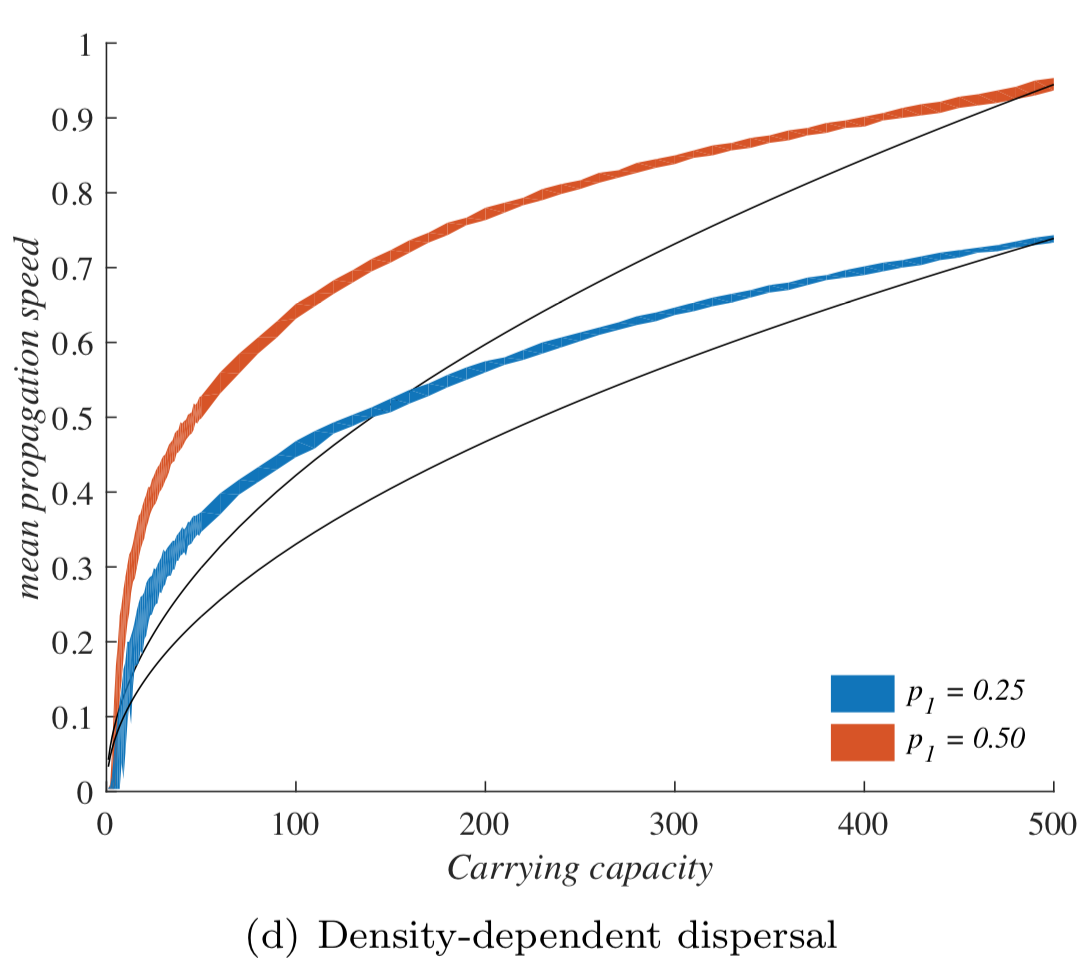
\includegraphics[scale=0.5]{fig.png}
  \label{Fig1}
\end{figure}
%%%%%%%%%%%%%%%%%%%%%%%%%%%%%%%%%%%%%%%%%%%%%%%%%%%%%%%%%%%%%%%%%%%%%%%%%%%%%%%%%%%%%%

\section*{Discussion}
Overall, this study carries a simple and clear message, supported by valuable contributions from different angles. Although some sections are clearly written for the theoretical ecology crowd, this article has something for everyone, from the stray physicist to the open-minded manager. The collaboration between theoreticians and experimentalists, while not central, is worthy of note. Because the narrative of this study is the variety of mechanisms that can lead to the same qualitative effect, the inclusion of various approaches is not a gimmick, but helps drive home its main message. The work is fairly self-contained, although one could always wish for further developments, especially in the direction of more quantitative testing of these mechanisms. \\ 

In conclusion, \textcite{levins1971regional} effectively convey the widely relevant message that, for some species, invading is not just about the destination, it is about the many offspring one makes along the way. \\ 


\section*{Acknowledgements}
This is your acknowledgments. Version \version~ of this article has been peer-reviewed and recommended by 
\emph{\PCI} (\DOIrecommendationlink)

\section*{Conflict of interest disclosure}
The authors of this preprint declare that they have no financial conflict of interest with the content of this article. XXX and XXX are recommenders for PCI XXX

\section*{Data, script and code availability}
Data are available online: link or DOI of the webpage hosting the data

\section*{Supplementary information availability}
Script and codes are available online: link or DOI of the webpage hosting the script and codes

\titleformat*{\section}{\bfseries\Large\centering}

\printbibliography[notcategory=ignore]

\section*{Annexes or Supplementary Information}
This is your annex 1 

This is your annex 2 

\end{document}
